\documentclass{article}
\usepackage[utf8]{inputenc}
\title{Homework}
\author{Mateusz Wyszecki}
\date{May 2019}

\usepackage{tipa}
\usepackage[T1]{fontenc}
\usepackage{phonrule}
\usepackage{qtree}
\usepackage{pgfplots}



\begin{document}
\maketitle
\newline




\section{My favourite topics in language studies and computer science:}

\begin{enumerate}
  \item Corpus stylistics
  \item Literary translation
  \item Sentiment analysis 
  \item Python programming
  \item SQL data-base management 
\end{enumerate}

\section{Phonetic Transcription}
\newline

\textdoublepipe{} ma\textsci \, ne\textsci m \textsci z \textprimstress m\ae \texttheta ju\textlengthmark \textdoublepipe{} a\textsci \, \textschwa m \textschwa \,  \textprimstress stju\textlengthmark d\textschwa nt \textturnscripta v \textprimstress n\ae \textteshlig r\textschwa l \textprimstress l\ae \ng w\textsci \textdyoghlig \, \textprimstress pr\textschwa \textupsilon s\textepsilon s\textsci \ng \,  \ae nd a\textsci \, \ae m \textprimstress ra\textsci t\textsci \ng \,  ma\textsci \,  \textprimstress m\textscripta \textlengthmark st\textschwa \,  \textprimstress \texttheta i\textlengthmark s\textsci s \textschwa \textprimstress ba\textupsilon t \textschwa \,  \textprimstress k\textopeno \textlengthmark p\textschwa s \, be\textsci st sta\textsci \textprimstress l\textsci st\textsci k \textprimstress st\textturnv di \textturnscripta v \textprimstress m\textturnscripta d\textschwa n \textprimstress sa\textsci \textschwa ns\textprimstress f\textsci k\textesh \textschwa n \textprimstress l\textsci t\textschwa r\textsci \textteshlig \textschwa \textdoublepipe{}  a\textsci \,  \textschwa m \textprimstress \textopeno \textlengthmark ls\textschwa \textupsilon  \, \textprimstress \textsci ntr\textsci st\textsci d \textsci n \textprimstress l\textsci t\textschwa r\textschwa ri tr\ae ns\textprimstress le\textsci \textesh \textschwa n \textdoublepipe{}
\newline
\newline
\textipa{ \textdoublepipe{}na"\textsubbridge{z}\textbari{}vAm "CE mA"\textsubbridge{t}Eu\textesh \textdoublepipe{} "jE\textsubbridge{s}\textsubbridge{t}Em \textsubbridge{s}\textsubbridge{t}u"\textsubbridge{d}En\textsubbridge{t}Em p\textesh  E\textsubbridge{t}fA"\textyogh A\textltailn{}A j\~{\textepsilon}"\textsubbridge{z}\textbari{}kA nA\textsubbridge{t}urAl"nEg\textopeno \textdoublepipe{} v "rAmAx "m\textopeno jEj "prA\texttoptiebar{t\textsubbridge{s}}\textbari{} mAg\super ji"\textsubbridge{s}\textsubbridge{t}Er\textsubbridge{s}k\super jjEj "pi\textesh E \textopeno \, k\textopeno rpu"\textsubbridge{s}\textopeno vEj A\textsubbridge{n}A"l\super ji\textctz E li\textsubbridge{t}ErA"\textsubbridge{t}ur\textbari \, sa\textsci \textschwa ns\textprimstress f\textsci k\textesh \textschwa n\textdoublepipe{}}

\newline


\section{A Syntactic Tree}
\Tree [.CP [.C' [.C {[decl.]} ] [.TP [.DP [.D' [.D This ] [.NP [.N' [.N tree ] ] ] ] ] [.T' [.T {[past]} ] [.VP [.V' [.V was ] [.DP [.D' [.D a ] ] [.NP [.N' [.N' [.N pain ] [.CP [.C' [.C {[decl.]} ] [.TP \qroof{PRO}.NP [.T' [.T to ] [.VP [.V' [.V draw ] ] ] ] ] ] ] ] [.PP [.P' [.P in ] [.DP [.D' [.D the ] [.NP  [.N' [.N neck ] ] ] ] ] ] ] ] ] ] ] ] ] ] ] ]

\section{Phonological Rules}
\newline
\textbf{Spirantization}

\newline
\phonb{\phonfeat{+stop \\ -voice} }{\phonfeat{+voice \\ -stop \\ +fricative} }{\phonfeat{+vowel}}{\phonfeat{+vowel} }
\newline
\newline
\textbf{Postnasal Voicing}

\newline
\newline
\phonb{\phonfeat{+stop}}{\phonfeat{+voice} }{\phonfeat{+nasal}}
\newline
\newline
\textbf{Nasalization}

\newline
\newline
\phonb{\phonfeat{+vowel}}{\phonfeat{+nasal}}{{}}{\phonfeat{+nasal}}
\newline
\newline
\textbf{Nasal Consonant Shortening}

\newline
\newline
\phonb{\phonfeat{+consonant \\ +nasal }}{\phonfeat{+short} }{{}}{\phonfeat{+consonat \\ -voice}}

\section{Mathematical Equation}
\newline
\newline
Similarity measure for syntactic trees:
\newline
\newline
\begin{math}
S_{TO}(T_{1},T_{2}) = \frac{max}{n_{1} \in nodes(T_{1}),n_{2} \in nodes(T_{2})}C_{TO}(n_{1},n_{2})
\end{math}
\newline
\newline
Sum of operation on syntactic trees:
\newline
\begin{math}

\noindent \gamma_{(S)} = \sum_{i=1}^{|S|} \gamma_{(S_{i})} 
\end{math}
\newline

\noindent Source: \textit{Mathematical Equation Structural Syntactical Similarity Patterns: A Tree
Overlapping Algorithm and Its Evaluation} by Evgeny Pyshkin 

\section{Pgfplots package}
Pgfplots is an advanced package used for creating both 2D and 3D graphs. The graphs are of high quality, but compiling them requires a great deal of processing power. Here are some examples of what Pgfplots can do: 

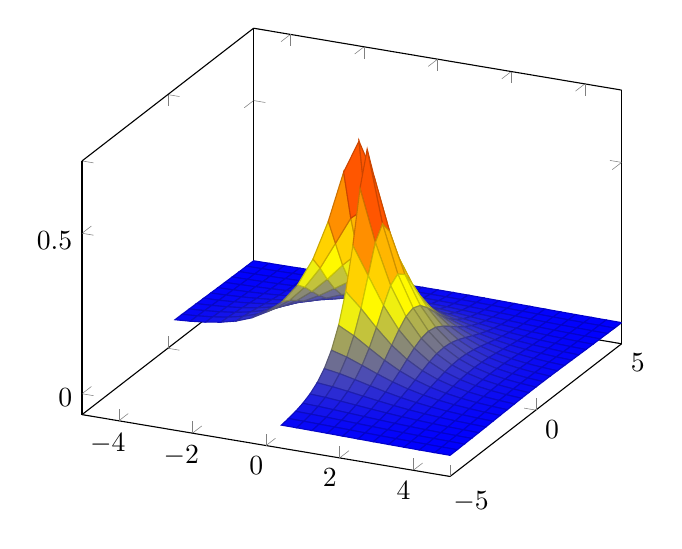
\begin{tikzpicture}
\begin{axis}[
unbounded coords=jump,
x filter/.expression={
x<0 && y<0 ? nan : x
},
]
\addplot3 [surf] {exp(-sqrt(x^2 + y^2))};
\end{axis}
\end{tikzpicture}

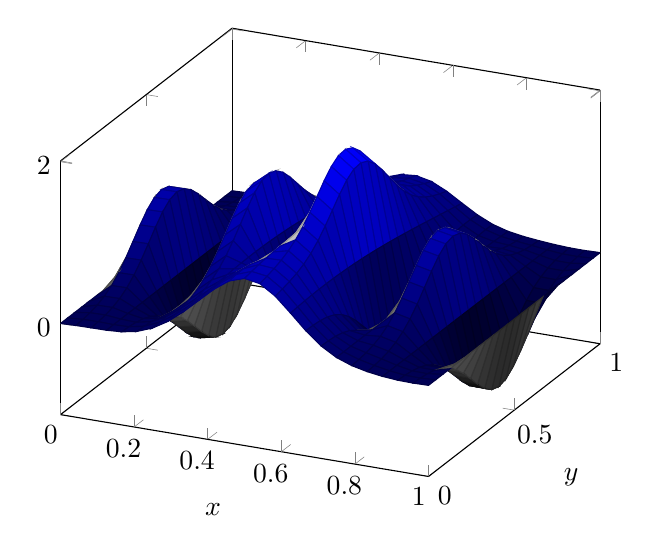
\begin{tikzpicture}
\begin{axis}[
title=,
xlabel=$x$,
ylabel=$y$,
]
\addplot3 [surf,
mesh/interior colormap={blueblack}{
color=(black) color=(blue)
},
colormap/blackwhite,
domain=0:1,
] {
sin(deg(8*pi*x))* exp(-20*(y-0.5)^2)
+ exp(-(x-0.5)^2*30
- (y-0.25)^2 - (x-0.5)*(y-0.25))
};
\end{axis}
\end{tikzpicture}

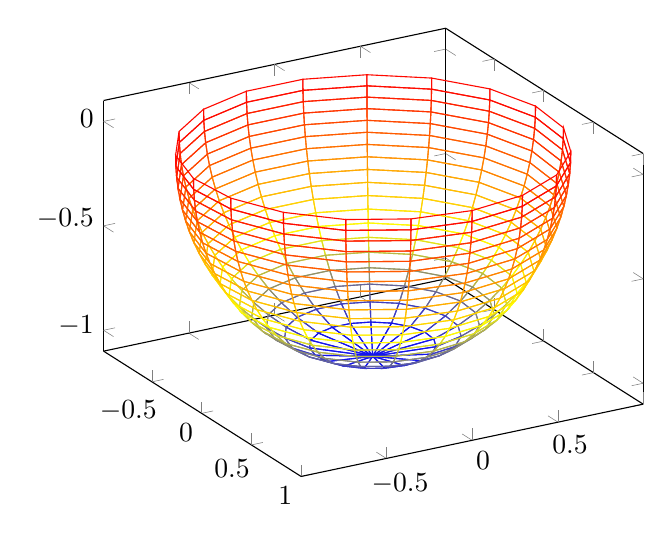
\begin{tikzpicture}
\begin{axis}[view={60}{30}]
\addplot3 [
mesh,
z buffer=sort,
samples=20,
domain=-1:0,
y domain=0:2*pi,
] (
{sqrt(1-x^2) * cos(deg(y))},
{sqrt( 1-x^2 ) * sin(deg(y))},
x
);
\end{axis}
\end{tikzpicture}

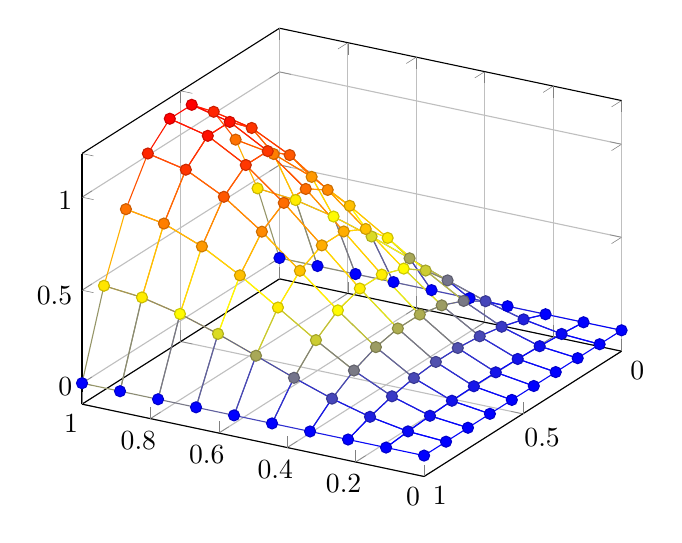
\begin{tikzpicture}
\begin{axis}[
grid=major,
view={210}{30},
]
\addplot3+ [
mesh,
scatter,
samples=10,
domain=0:1,
] {5*x*sin(2*deg(x)) * y*(1-y)};
\end{axis}
\end{tikzpicture}



\end{document}

